%Some basic ways to manipulate text are \textit{italics} and \textbf{bold}. One can reference Figures (see Figure \ref{fig:taltech} for an example) as well as cite references which are defined in the \textit{references.bib} file.\cite{spectre,example-reference}
%
%The \textit{Bibliography}, \textit{List of Figures} and \textit{List of Tables} are all automatically generated and references will be updated automatically as well. This means that if you've defined a citation but are not referencing it, it will not appear in the \textit{Bibliography}. This also means that any Figure / Table / Citations numbers are automatically updated as well. Numbering is done by order-of-appearance.
%
%One can create an itemized list:
%\begin{itemize}
%    \item item a
%    \item item b
%    \item ...
%\end{itemize}
%
%Or enumerate them:
%\begin{enumerate}
%    \item item x
%    \item item y
%    \item ...
%\end{enumerate}
%
%
%\begin{figure}[ht]
%    \centering
%    
\includegraphics[width=.5\textwidth]{figures/taltech.jpg}
%    \caption{\textit{An image of the TalTech logo.}}
%    \label{fig:taltech}
%\end{figure}
%
%
%A table with three columns can be seen in Table \ref{tab:requirements}.
%\begin{longtable}{|p{0,5cm}|p{10cm}|p{3cm}|}
%	\caption{\it{A table with some requirements}}
%	\label{tab:requirements}\\ \hline
%	\textbf{Nr} &  \textbf{Requirement} & \textbf{Weight}  \\
%	\hline
%	\endfirsthead
%	\multicolumn{3}{l}%
%	{\tablename\ \thetable\ -- \textit{Continues...}} \\ q
%	\hline
%	\textbf{Nr} &  \textbf{Requirement} & \textbf{Importance}  \\
%	\hline
%	\endhead
%	\hline \multicolumn{3}{l}{\textit{Continues...}} \\
%	\endfoot
%	\hline
%	\endlastfoot
%1 & Price & High\\ \hline
%2 & Variety& Middle\\ \hline
%3 & Support& Low\\ \hline
%
%\end{longtable}
%
%We can use variables set in the \textit{main.tex} file to render values like our title (\doctitle) or supervisor names (\textbf{Supervisor}: \supervisor, \textbf{Co-supervisor}: \cosupervisor{}).
%\section{What is a stream processing}\label{sec:stream-beg}
%Stream processing
%
%\section{Brief history of stream processing systems}\label{sec:breif-history}
%Stream processing


\section{Background and Motivation}\label{sec:back-and-motiv}
Software engineering is a diverse field that addresses various business domain problems.
These domain-specific issues and their corresponding use cases necessitate in-depth analysis to determine the most suitable technologies for achieving optimal problem-solving outcomes.
One rapidly growing area in software engineering is big data.
Although big data is sometimes regarded as a marketing term, it encompasses complex data processing frameworks and datasets.

As the volume of produced data has dramatically increased over the years, modern technical solutions capable of processing massive amounts of data are required.
The open-source community offers decent frameworks and tools, making it challenging to choose the best option.
This research focuses on comparing the most suitable frameworks for specific use cases, particularly those that are designed for stateful real-time stream processing.

Stream processing use cases are relatively rare compared to typical problems that can often
be solved with traditional batch processing or simple programs that don't require the MapReduce model.
However, stateful stream processing assumes that real-time processing relies on previous states and unbounded data flow, which may indicate abnormal system behavior, such as fraud alerts in financial transactions
within a specific time frame.
Quick response can facilitate necessary actions and save time.
Therefore, it is crucial to provide a technical analysis of the most suitable frameworks, assess their advantages and disadvantages, and examine the complexities involved in their application for stateful stream processing based on a given use case.
This master's thesis offers a technical overview, benchmarks, and comparisons for appropriate use cases.
The use case considers that incoming events trigger state aggregation and re-computation and evaluates how efficiently Kafka Streams \cite{kafka_streams_intro} and Apache Flink \cite{flink_intro} manage the state under heavy loads, represented by a stream of Kafka \cite{kafka_intro} messages.
The ideal framework should address existing problems while offering excellent scalability, state recovery, and cost efficiency.

\newpage
\section{Problem Statement}\label{sec:prob-st}
The problem comes with business demands that are based on current needs for a more scalable and efficient solution.
Before getting into the problem details, the current model will be provided to better understand why this research
brings value and how streaming frameworks are comparable with the batch processing model \ref{fig:current-model}.

\subsection{Batch Processing Model Overview}\label{subsec:current-model}

\begin{figure}[ht]
    \centering
    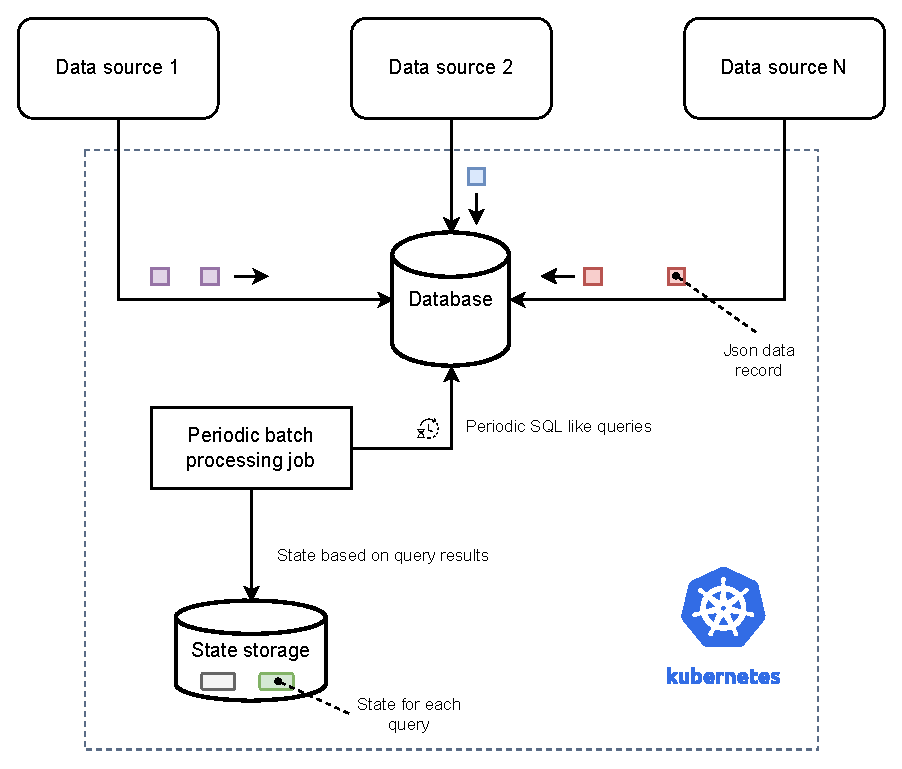
\includegraphics[width=1\textwidth]{figures/current-model-2}
    \caption{\textit{Generic model of a batch processing job that should replaced by stateful stream processing.}}
    \label{fig:current-model}
\end{figure}

%Compo.

\begin{description}
    \item[Kubernetes] Open source platform for managing containerized workloads and services \cite{kubernetes_intro}.
    \item[Data course N] It is an external data source component that sends a json records as unbounded stream.
    \item[Batch processing job] Represents a worker that executes queries in the databsase
     and saves a query result as a state to the state database.
    It runs with a predefined interval.
    \item[State storage] Is a storage for states.
    Each query has its own state.
    \item[Database] Stores records from data sources.
\end{description}

%From a first look, the system on the Figure \ref{fig:current-model} represens a straightforward
%architecture.
%Generally, the systems that implement such an architecture are easily debuggable,
%testable and quite often are a good way to go when the project gets started.
%Everything might work smoothly for ages.
%At some moment in time, the system might face with a breaking point which brings new challenges.
%
%For example, in a few years, the number of data sources has significantly grown, where each
%data source has its own sending frequency and a type.
%A new load would require adding more and more instances of a job, faster period of job execution.
%And also it leads to additional types of errors to handle, which haven't been seen before.
%An execution of each query gets more expensive.
%Not every data can be indexed, and especially if the amount of indexed data has grown in many times, it adds
%a significant complexity overhead for a query execution.
%Moreover, additional errors might and circumstances may get the service down, which requires
%additional balancing logic and a state recovery.
%It might take a significant time to recover a service in a specific region if this requires a manual work
%from an engineering team.

Some of the main disadvantages of the batch proccessing illustrated on Figure \ref{fig:current-model}l.
New stateful stream processing with Kafka Stream and Apache Flink should overcome these disadvantages,
and provide a brand-new solution to process unbound data streams.

\begin{itemize}
    \item The system is not scalable enough.
    \item The state gets lost it the job gets killed.
    \item Periodic batch processing has higher latency compared to stream proccesig that is designed to
    proccess data in real time with a minimal latency.
\end{itemize}

%\newpage
\section{Research Question and Objectives}\label{sec:res-q-o}
The main question is to figure out how different frameworks behave in case of fault tolerance,
for example, if some processing replicas or workers get killed.
How would load rebalancing work, how much delay would it create,
and how long would it take for the system to restore a state?
The research consists of several tasks.

\begin{itemize}
    \item Create prototypes with Apache Flink and Kafka Streams.
    \item Prepare cloud setup to make experiments repeatable.
    \item Define metrics and benchmarks.
    \item Execute experiments.
    \item Collect results for analysis.
    \item Plot the data and make a conclusion.
\end{itemize}


\subsection{Selecting a Suitable Framework}\label{subsec:selecting-a-suitable-framework}
They're lots different frameworks out there available for solving different
data streaming problems.
Most of the frameworks were born on top of each other as a new generation solution \cite{fragkoulis2023survey}.
Each new framework is trying to bring better performance and scalability.
Down below is an evolution of streaming frameworks \cite{stream_processing_history} with a brief description:

\begin{description}
    \item[Apache S4]  Apache S4 (Simple Scalable Streaming System) was an early stream
    processing engine developed at Yahoo! Labs.
    It was designed for unbounded data stream processing which uses
    simple programming model based on a publish/subscribe pattern.
    Apache S4 became an open source project under Apache Software Foundation but
    eventually became inactive due to limited community adoption \cite{apache_s4_intro}.
    \item[Apache Storm]
    Apache Storm was a popular distributed stream processing framework.
    It was designed for real-time data processing and provided guarantees such as
    at-least-once and exactly-once processing semantics.
    Apache Storm was more popular comparing to Apache S4, but it provides less
    performance and flexibility comparing to next generation frameworks \cite{apache_storm_performance}.
    \item[Apache Flink] Originally was developed at the Technical University of Berlin.
    Apache Flink is one of the most powerful stream processing framework that unified batch and
    stream processing with focusing on streaming.
    Flink provided low-latency, high-throughput, and exactly-once processing semantics.
    With its advanced features, such as event time processing, watermarks, and savepoints,
    Flink has become the one of the most popular stream processing framework which is
    well-designed for highly loaded complex data stream processing use cases \cite{flink_intro}.
    \item[Kafka Streams] Introduced as part of Apache Kafka, Kafka Streams
    is a rather a stream processing library than a framework which allows developers to build real-time
    applications and microservices using the Kafka platform.
    Kafka Streams provides a simple, functional programming model and is tightly
    integrated with the Kafka ecosystem.
    It's well-suited for use cases like real-time analytics, data transformation
    and event-driven architectures.
    Kafka Stream can a replacement for Apache Flink for cases where heavy integration
    and complex computation is not needed \cite{kafka_streams_intro}.
    \item[Apache Spark] Is well known alternative for Apache Flink and Kafka Streams,
    is a popular solution for most of the cases, but does a micro-batching \cite{spark_structured_streaming}.
\end{description}

However, for this study Apache Flink and Kafka streams were chosen as most popular real-time processing
framework which do not use micro-batching.

\subsection{Deployment Environment}\label{subsec:deployment-environment}
In 2024, the most popular and advanced application container manager is Kubernetes.
First, stream processing frameworks were designed to be run on YARN clusters.
YARN is no longer considered to be the preferred deployment manager.
It means that a framework must be able to run in Kubernetes using containers.
All experiments for this study were conducted with an AWS cloud provider.


\subsection{Requirements Summary}\label{subsec:final-requirements}
Apache Flink and Kafka Streams are two leading stream processing frameworks
that are used in prototypes.

As a summary, these important bullet points provided down below which will
be considered during the evaluation for the new solution.

\begin{description}
    \item[Scalability] The current is not scalable enough.
    \item[Fault tolerance] A state must not be lost if a pod where a running job gets killed.
    The system should be able to proceed stream processing with previous state once job is restarted.
    \item[Simple integration] A solution, weather it is a programming language,
    or framework, should be compatible with the current technology stack, such as JVM and Kubernetes.
    It also means that a solution won't require hiring an entire engineering department or a team.
    \item[Cost effecienty] It's quite important that a highly loaded solution doesn't cost too much.
    \item[Cloud independence] A solution must not depend on a cloud provider.
    \item[Functionality] A solution has to have an API that allows to implement and test a considered use case.
\end{description}


